% Minimal or maximal Spanning Trees
\begin{figure}[htb]
\centering
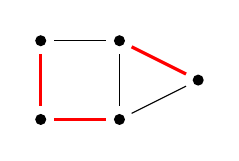
\begin{tikzpicture}[every node/.style = {circle}]

\node (a) at (0,0) {};
\node (b) at (1,0) {};
\node (c) at (2,0.5) {};
\node (d) at (1,1) {};
\node (e) at (0,1) {};
\foreach \node in {a,...,e}
{
	\fill (\node) circle [radius=2pt];
};

\draw[red,very thick] (a) -- (b);
\draw[red,very thick] (a) -- (e);
\draw[red,very thick] (c) -- (d);
%\draw (a) -- (b);
%\draw (a) -- (e);
\draw (b) -- (c);
\draw (b) -- (d);
%\draw (c) -- (d);
\draw (d) -- (e);
\end{tikzpicture}
\caption{Graph $G$ and its maximal spanning forest}
\end{figure}



